\documentclass[11pt,a4paper]{article}

% --- Essential Packages ---
\usepackage[utf8]{inputenc}
\usepackage[T1]{fontenc}
\usepackage{times}
\usepackage[margin=1in]{geometry}
\usepackage{microtype}
\usepackage{amsmath,amssymb,amsfonts,amsthm}
\usepackage{booktabs}
\usepackage{makecell}
\usepackage{adjustbox}
\renewcommand\theadfont{\bfseries\small}
\renewcommand\theadalign{cc}
\setlength{\tabcolsep}{5pt}
\usepackage{tabularx}
\usepackage{longtable}
\usepackage{array}
\usepackage{multirow}
\usepackage{graphicx}
\usepackage{xcolor}
\usepackage{tikz}
\usetikzlibrary{shapes,arrows.meta,positioning,calc,fit,backgrounds}
\usepackage{tcolorbox}
\usepackage{enumitem}
\usepackage{caption}
\usepackage{subcaption}
\usepackage[numbers,sort&compress]{natbib}
\usepackage[breaklinks=true,colorlinks=true,linkcolor=blue!70!black,citecolor=blue!70!black,urlcolor=blue!70!black]{hyperref}
\usepackage{cleveref}

% --- Custom Formatting & Commands ---
\newcolumntype{L}[1]{>{\raggedright\let\newline\\\arraybackslash\hspace{0pt}}m{#1}}
\newcolumntype{C}[1]{>{\centering\let\newline\\\arraybackslash\hspace{0pt}}m{#1}}
\newcolumntype{R}[1]{>{\raggedleft\let\newline\\\arraybackslash\hspace{0pt}}m{#1}}
\newcolumntype{Y}{>{\centering\arraybackslash}X}

\tcbset{
    boxrule=0.75pt,
    colback=gray!5!white,
    colframe=gray!50!black,
    arc=3pt,
    left=6pt,right=6pt,top=6pt,bottom=6pt
}

\title{\textbf{\Large Calibrated Bipartite Matching for Perspective Coverage\\in Large Language Models}}

\author{
  \textbf{Dhruthika Thoutam} \\
  Indian Institute of Technology Gandhinagar \\
  \texttt{thoutam.dhruthika@iitgn.ac.in}
}

\date{\today}

\begin{document}

\maketitle

\begin{abstract}
When Large Language Models (LLMs) are deployed in deliberative, democratic, or decision-support environments, they must not collapse onto a single consensus stance; they must faithfully represent the full landscape of valid human perspectives. Evaluating perspective coverage requires determining whether a model's generated viewpoints capture the diverse reasons, values, and argumentative warrants established by human deliberators, rather than merely repeating superficial paraphrases. 

In this work, we introduce the \textbf{Calibrated Maximum Bipartite Matching Framework} for evaluating generative deliberation. Our framework pairs generated viewpoints with ground-truth human equivalence clusters through a calibrated two-stage pipeline: dense candidate retrieval ($\tau^* = 0.55$), uncertainty-preserving stance filtering, a fine-tuned cross-encoder warrant probe ($T^* = 0.20$), and the Kuhn--Munkres maximum-weight bipartite matching algorithm to enforce strict one-to-one correspondence.

Evaluating 34 open-source LLMs across 205,286 viewpoints on all 907 claims of the Perspectrum deliberation benchmark reveals four primary empirical findings:
\begin{enumerate}[leftmargin=*,itemsep=1pt]
    \item \textbf{Compact Models Excel Under Controlled Budgets:} When models are evaluated under a strictly standardized budget of $K = 5$ viewpoints per claim, \texttt{llama\_3\_2\_3b\_instruct} achieves the highest coverage (\textbf{54.90\%}, efficiency 0.512), significantly outperforming larger models including \texttt{llama\_3\_1\_8b\_instruct} (46.41\%, $p_{\text{adj}} < 10^{-17}$) and \texttt{gemma\_2\_27b\_it} (47.90\%, $p_{\text{adj}} < 10^{-12}$).
    \item \textbf{Budget-Bottlenecked vs. Parameter-Bottlenecked Coverage:} Empirical hypothesis testing demonstrates that perspective coverage under fixed budgets is \textbf{budget-bottlenecked rather than parameter-bottlenecked}. Merely scaling model weights without expanding the generation horizon ($K$) does not compel the model to uncover new perspectives: scaling from \texttt{gemma\_2\_9b\_it} to \texttt{gemma\_2\_27b\_it} ($\Delta = -0.0026$, $p = 0.633$), \texttt{olmo\_2\_7b\_inst} to \texttt{13b} ($p = 0.832$), and \texttt{llama\_3\_1\_8b} to \texttt{llama\_3\_3\_70b} ($p = 0.389$) all result in statistical parity.
    \item \textbf{Supervised Fine-Tuning Drives Perspective Diversity:} Across OLMo 2 architectures, Supervised Fine-Tuning (SFT) yields a massive $+9.57\%$ to $+18.02\%$ coverage increase over pre-trained base models ($p_{\text{adj}} < 10^{-13}$), while Direct Preference Optimization (DPO) further refines deliberative balance without collapsing perspective diversity ($+2.38\%$, $p < 0.01$).
    \item \textbf{Resolution of Multiplicity Ceilings:} On high-complexity claims ($\ge 7$ clusters), raw coverage for $K=5$ models drops to $\approx 41\%$ due to mathematical budget limits, but \textbf{Normalized Coverage ($NC_c$)} reaches \textbf{82.8\%--83.9\%}, demonstrating that models capture nearly all perspectives permitted by their generation budget.
\end{enumerate}
\end{abstract}

\vspace{0.5em}
\noindent\textbf{Keywords:} Perspective Coverage, Large Language Models, Generative Deliberation, Kuhn--Munkres Matching, Bipartite Graphs, Stance Verification, Perspectrum Benchmark.

\newpage

% =============================================================================
\section{Introduction and Problem Formulation}
\label{sec:introduction}
% =============================================================================

Evaluating Large Language Models on controversial, open-ended, or subjective topics requires assessing whether model outputs reflect the diverse landscape of valid human perspectives. In democratic discourse, civic debate, and policy deliberation, an AI assistant should not act as an advocate for a single ideological viewpoint; it should surface the multidimensional arguments surrounding a topic.

\subsection{What is Perspective Coverage?}
\label{subsec:perspective_coverage_def}
\textbf{Perspective coverage} measures the degree to which an LLM's generative output recovers the complete distribution of ground-truth human argumentative viewpoints associated with a given controversial claim. When evaluating perspective coverage, we must distinguish between four distinct concepts:
\begin{enumerate}[leftmargin=*,itemsep=2pt]
    \item \textbf{High-Volume Verbosity:} Producing many sentences that assert the same underlying point under slight lexical variations (e.g., \textit{``Solar energy reduces fossil fuel consumption''} and \textit{``Solar panels cut fossil fuel reliance''}).
    \item \textbf{Semantically Distinct Viewpoints:} Statements that introduce different topics but may lack a valid argumentative relationship to the central claim.
    \item \textbf{Recovery of Human Perspectives:} Generative arguments that successfully match the underlying reasons, values, and warrants established by human deliberative communities (represented in this work by the crowd-annotated equivalence clusters of Perspectrum).
    \item \textbf{Valid Extraneous Perspectives:} Legitimate human arguments that exist in the real world but happen to be absent from the reference benchmark. A benchmark evaluation captures \textit{relative recovery against a curated human standard}, not an exhaustive inventory of all possible human thoughts.
\end{enumerate}

\subsection{The Need for Calibrated Bipartite Matching}
\label{subsec:need_for_matching}

Standard similarity metrics often rely on greedy thresholding, allowing multiple generated sentences to match the same human perspective, or allowing a single generated sentence to claim credit for multiple distinct gold perspectives. This rewards verbose models that produce repetitive paraphrases while penalizing disciplined models that produce concise, atomic outputs.

To solve this, we formulate perspective evaluation as a \textbf{maximum-weight bipartite matching problem} over ground-truth equivalence clusters (\Cref{fig:bipartite_schematic}). Enforcing strict one-to-one correspondence ensures that:
\begin{itemize}[leftmargin=*,itemsep=1pt]
    \item Redundant paraphrases cannot claim duplicate credit.
    \item Models are evaluated on their ability to uncover distinct, non-overlapping argumentative warrants.
    \item Generative verbosity is disentangled from genuine perspective diversity.
\end{itemize}

\begin{figure}[htbp]
\centering
\begin{tikzpicture}[scale=0.95, every node/.style={transform shape}]
    % Greedy Box
    \node[draw=red!70!black, fill=red!5, rounded corners, thick, inner sep=8pt, text width=6.8cm] (greedy) {
        \textbf{\textcolor{red!70!black}{Unconstrained Greedy Matching (Flawed)}}\\[0.5em]
        \textbf{Generated Viewpoints ($V_h$)} \hfill \textbf{Gold Clusters ($C_g$)}\\[0.3em]
        \tikz \node[draw, fill=white, rounded corners, inner sep=3pt] (v1) {\small $h_1$: ``Cuts carbon emissions''}; \hfill
        \tikz \node[draw, fill=white, rounded corners, inner sep=3pt] (c1) {\small Cluster A: Emissions};\\[0.4em]
        \tikz \node[draw, fill=white, rounded corners, inner sep=3pt] (v2) {\small $h_2$: ``Lowers CO$_2$ output''}; \hfill
        \tikz \node[draw, fill=white, rounded corners, inner sep=3pt] (c2) {\small Cluster B: Economics};\\[0.6em]
        \draw[-{Stealth[length=2.5mm]}, red!70!black, thick] (v1.east) -- (c1.west);
        \draw[-{Stealth[length=2.5mm]}, red!70!black, thick, dashed] (v2.east) -- (c1.west);
        \centering\footnotesize\textcolor{red!80!black}{\textbf{Double-counts Cluster A! Rewards verbosity.}}
    };
    
    % Kuhn-Munkres Box
    \node[draw=green!60!black, fill=green!5, rounded corners, thick, inner sep=8pt, text width=6.8cm, right=1.2cm of greedy] (km) {
        \textbf{\textcolor{green!60!black}{Kuhn--Munkres Bipartite Matching (Ours)}}\\[0.5em]
        \textbf{Generated Viewpoints ($V_h$)} \hfill \textbf{Gold Clusters ($C_g$)}\\[0.3em]
        \tikz \node[draw, fill=white, rounded corners, inner sep=3pt] (kv1) {\small $h_1$: ``Cuts carbon emissions''}; \hfill
        \tikz \node[draw, fill=white, rounded corners, inner sep=3pt] (kc1) {\small Cluster A: Emissions};\\[0.4em]
        \tikz \node[draw, fill=white, rounded corners, inner sep=3pt] (kv2) {\small $h_2$: ``Lowers CO$_2$ output''}; \hfill
        \tikz \node[draw, fill=white, rounded corners, inner sep=3pt] (kc2) {\small Cluster B: Economics};\\[0.6em]
        \draw[-{Stealth[length=2.5mm]}, green!60!black, very thick] (kv1.east) -- (kc1.west);
        \centering\footnotesize\textcolor{green!70!black}{\textbf{Strict 1-to-1 Injection: No duplicate credit.}}
    };
\end{tikzpicture}
\caption{\textbf{Comparison of matching paradigms.} Left: Greedy matching allows redundant paraphrases to claim duplicate credit. Right: Kuhn--Munkres maximum-weight bipartite matching enforces strict injectivity.}
\label{fig:bipartite_schematic}
\end{figure}

% =============================================================================
\section{The Perspectrum Deliberation Benchmark}
\label{sec:perspectrum_dataset}
% =============================================================================

\subsection{Dataset Topology}
\label{subsec:dataset_topology}
We utilize the complete Perspectrum deliberation benchmark \citep{chen2019perspectrum}, processed via \texttt{src/data\_prep/parse\_perspectrum.py}:
\begin{itemize}[leftmargin=*,itemsep=1pt]
    \item \textbf{Claims ($N_{\text{claims}} = 907$):} Controversial societal, legal, moral, and political propositions (e.g., \textit{``Mandatory military service should be instituted''}).
    \item \textbf{Gold Perspective Clusters ($N_{\text{clusters}} = 5,095$):} Ground-truth semantic equivalence clusters ($\mu = 5.62$ clusters per claim; range: $1 \dots 16$). Matching \textit{any} single human statement within a cluster grants coverage for that cluster.
    \item \textbf{Human Perspective Instances ($N_{\text{perspectives}} = 11,805$):} Crowd-annotated statements ($\mu = 2.32$ paraphrases per cluster).
    \item \textbf{Stance Distribution:} 6,112 Support ($51.77\%$) vs. 5,693 Undermine ($48.23\%$).
    \item \textbf{The Evaluation Denominator:} All full-corpus coverage metrics use the \textbf{5,095 gold perspective clusters} as the denominator.
\end{itemize}

\subsection{Structure of a Debate Claim and Equivalence Clusters}
A single debate claim encompasses multiple distinct perspective clusters across opposing stances. For example, for Claim \#204 (\textit{``Social media does more harm than good for teenage mental health''}):
\begin{itemize}[leftmargin=*,itemsep=1pt]
    \item \textbf{Gold Cluster A (Stance: SUPPORT):} Core Warrant: \textit{Algorithmic social comparison and cyberbullying}. Paraphrases include: \textit{``Platforms promote unrealistic body standards''} and \textit{``Teens face constant algorithmic social comparison.''}
    \item \textbf{Gold Cluster B (Stance: UNDERMINE):} Core Warrant: \textit{Community support for marginalized youth}. Paraphrases include: \textit{``Online groups provide peer support for LGBTQ+ youth''} and \textit{``Isolated youth find belonging in digital groups.''}
\end{itemize}

% =============================================================================
\section{Model Inventory and Generation Protocol}
\label{sec:model_inventory}
% =============================================================================

\subsection{Model Inventory Across Four Generation Tiers}
We evaluated \textbf{34 open-source LLMs} spanning parameter scales from 135M to 32.5B across five major model families (Qwen 2.5, Llama 3, Gemma 2, OLMo 2, and SmolLM 2). Viewpoint generation was frozen in \texttt{data/viewpoint\_separated/production\_freeze\_manifest.json}, yielding \textbf{205,286 total viewpoints}. Models are classified into four empirical generation-budget tiers (\Cref{tab:generation_tiers}).

\begin{table*}[htbp]
\centering
\small
\caption{\textbf{Inventory of 34 Evaluated Language Models Categorized into Four Generation-Budget Tiers.} Viewpoint generation budget determines the operational ceiling of raw coverage.}
\label{tab:generation_tiers}
\begin{adjustbox}{max width=\textwidth}
\begin{tabular}{l c c p{5.5cm} p{7.2cm}}
\toprule
\textbf{Generation Tier} & \makecell{\textbf{Total Viewpoints}\\\textbf{($N_{\text{vp}}$)}} & \makecell{\textbf{Mean}\\\textbf{$K_c$}} & \textbf{Models Included} & \textbf{Generation Characteristics} \\
\midrule
\textbf{Tier 1: High-Volume} & 10,000--19,000 & 12.1--20.5 & \texttt{qwen2\_5\_32b\_instruct}, \texttt{smollm2\_135m\_instruct}, \texttt{qwen2\_5\_1\_5b\_instruct}, \texttt{qwen2\_5\_3b\_instruct} & Multi-sentence sub-arguments per prompt turn; high raw coverage but lower efficiency ($0.17$--$0.33$). \\
\addlinespace
\textbf{Tier 2: Elevated/Base} & 5,000--9,999 & 6.9--8.3 & \texttt{smollm2\_360m\_instruct}, \texttt{olmo\_2\_0425\_1b}, \texttt{olmo\_2\_1124\_7b}, \texttt{olmo\_2\_1124\_13b}, \texttt{olmo\_2\_0325\_32b} & Base pre-trained models lacking chat termination tokens; continue generating past 5 turns. \\
\addlinespace
\textbf{Tier 3: Standard Budget} & 4,400--4,700 & 5.0 & 22 Models: \texttt{llama\_3\_2\_3b}, \texttt{olmo\_2\_7b\_inst}, \texttt{gemma\_2\_9b}, \texttt{olmo\_2\_13b\_inst}, \texttt{gemma\_2\_27b}, \texttt{llama\_3\_1\_8b}, \texttt{qwen2\_5\_7b\_p2}, etc. & Strictly adhered to 5-step aspect history ($K = 5$ viewpoints per claim). Standardized benchmark. \\
\addlinespace
\textbf{Tier 4: Abstention-Heavy} & $<$ 4,400 & $<$ 4.0 & \texttt{qwen2\_5\_14b\_instruct\_p2}, \texttt{qwen2\_5\_3b\_instruct\_p2} & Phase 2 structured aspect prompting with abstention; models actively abstained on 36.7\%--66.0\% of queries. \\
\bottomrule
\end{tabular}
\end{adjustbox}
\end{table*}

\subsection{Multi-Turn Aspect Prompting Protocol}
Generations were elicited through a structured, multi-turn protocol across \textbf{5 Canonical Deliberative Aspects}: \textit{Economic}, \textit{Moral}, \textit{Legal}, \textit{Practical}, and \textit{Social}. Prompts enforced:
\begin{enumerate}[leftmargin=*,itemsep=1pt]
    \item \textbf{$K$-Step Generation History:} At each step $k \in \{0 \dots 4\}$, the model received the claim, the assigned aspect, and its own previous arguments for that claim.
    \item \textbf{Semantic Novelty Constraint:} Explicitly instructed that a paraphrase of an earlier point does not qualify as a new perspective.
    \item \textbf{Structured Abstention:} If no valid argument existed under an aspect, the model produced an explicit JSON abstention object (\texttt{"status": "abstain"}).
    \item \textbf{Sampling Parameters:} Temperature $T = 0.80$, Top-$p = 0.95$, Max New Tokens = 256, Repetition Penalty = 1.05. Fixed per-step random seed ($\text{seed} = 42 + \text{step}$).
\end{enumerate}

% =============================================================================
\section{The Calibrated Matching and Verification Architecture}
\label{sec:pipeline}
% =============================================================================

The evaluation pipeline processes generated viewpoints through four sequential stages (\Cref{fig:pipeline_flowchart}):

\begin{figure*}[htbp]
\centering
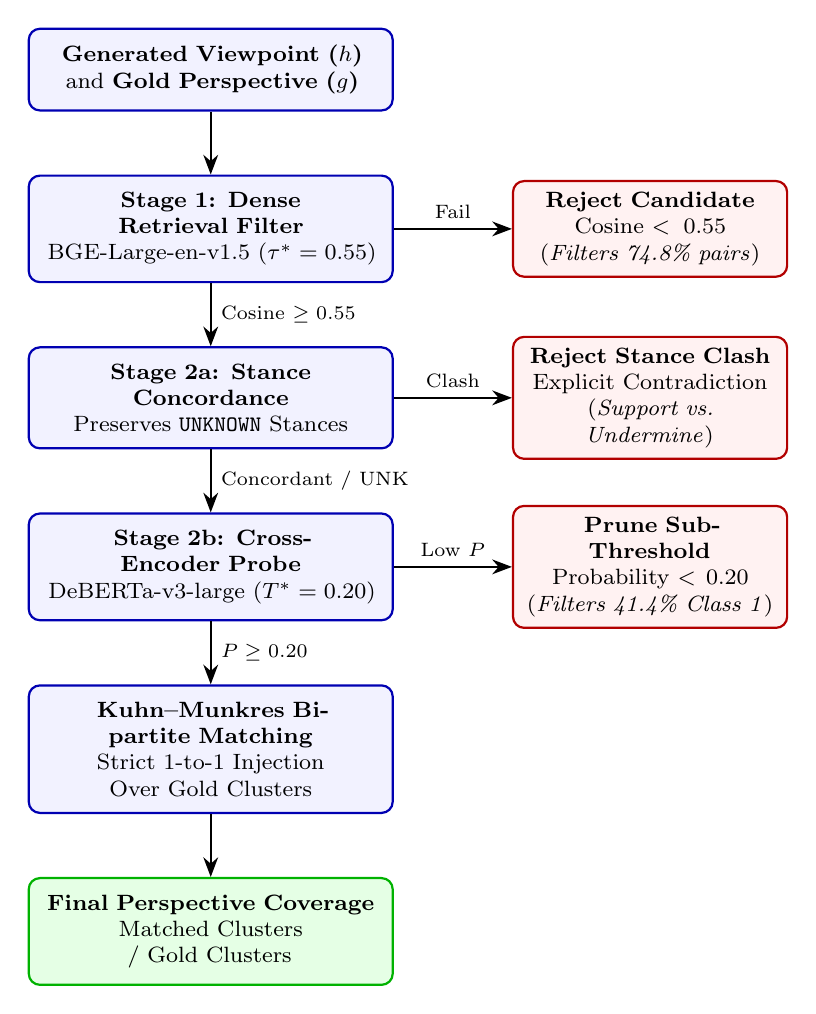
\begin{tikzpicture}[
    node distance=0.8cm and 1.2cm,
    every node/.style={font=\footnotesize},
    block/.style={rectangle, draw=blue!70!black, fill=blue!5, rounded corners, thick, text width=4.2cm, align=center, inner sep=6pt},
    reject/.style={rectangle, draw=red!70!black, fill=red!5, rounded corners, thick, text width=3.2cm, align=center, inner sep=4pt},
    arrow/.style={-{Stealth[length=2.5mm]}, thick}
]
    % Main Stages
    \node[block] (input) {\textbf{Generated Viewpoint ($h$)}\\and \textbf{Gold Perspective ($g$)}};
    \node[block, below=of input] (stage1) {\textbf{Stage 1: Dense Retrieval Filter}\\BGE-Large-en-v1.5 ($\tau^* = 0.55$)};
    \node[reject, right=1.5cm of stage1] (rej1) {\textbf{Reject Candidate}\\Cosine $< 0.55$\\(\textit{Filters 74.8\% pairs})};
    
    \node[block, below=of stage1] (stage2a) {\textbf{Stage 2a: Stance Concordance}\\Preserves \texttt{UNKNOWN} Stances};
    \node[reject, right=1.5cm of stage2a] (rej2a) {\textbf{Reject Stance Clash}\\Explicit Contradiction\\(\textit{Support vs. Undermine})};
    
    \node[block, below=of stage2a] (stage2b) {\textbf{Stage 2b: Cross-Encoder Probe}\\DeBERTa-v3-large ($T^* = 0.20$)};
    \node[reject, right=1.5cm of stage2b] (rej2b) {\textbf{Prune Sub-Threshold}\\Probability $< 0.20$\\(\textit{Filters 41.4\% Class 1})};
    
    \node[block, below=of stage2b] (stage3) {\textbf{Kuhn--Munkres Bipartite Matching}\\Strict 1-to-1 Injection Over Gold Clusters};
    \node[block, below=of stage3, fill=green!10, draw=green!70!black] (output) {\textbf{Final Perspective Coverage}\\Matched Clusters / Gold Clusters};
    
    % Connections
    \draw[arrow] (input) -- (stage1);
    \draw[arrow] (stage1) -- node[above]{\scriptsize Fail} (rej1);
    \draw[arrow] (stage1) -- node[right]{\scriptsize Cosine $\ge 0.55$} (stage2a);
    \draw[arrow] (stage2a) -- node[above]{\scriptsize Clash} (rej2a);
    \draw[arrow] (stage2a) -- node[right]{\scriptsize Concordant / UNK} (stage2b);
    \draw[arrow] (stage2b) -- node[above]{\scriptsize Low $P$} (rej2b);
    \draw[arrow] (stage2b) -- node[right]{\scriptsize $P \ge 0.20$} (stage3);
    \draw[arrow] (stage3) -- (output);
\end{tikzpicture}
\caption{\textbf{The Cascaded Perspective Matching and Verification Pipeline.} Candidate pairs pass sequentially through dense bi-encoder retrieval, stance concordance filtering, cross-encoder warrant probing, and Kuhn--Munkres maximum-weight bipartite matching.}
\label{fig:pipeline_flowchart}
\end{figure*}

\subsection{Stage 1: Dense Candidate Retrieval}
\label{subsec:stage1}
Pairs are embedded using \texttt{BAAI/bge-large-en-v1.5} (1,024 dimensions). We compute pairwise cosine similarity:
\begin{equation}
\text{sim}_{\text{cos}}(h, g) = \frac{\mathbf{e}_h \cdot \mathbf{e}_g}{\|\mathbf{e}_h\| \|\mathbf{e}_g\|}
\end{equation}

\subsubsection{Motivation and Theoretical Selection of BGE-Large}
Developed by the Beijing Academy of Artificial Intelligence \citep{xiao2023bge}, BGE-Large is among the highest-ranking open-source models on the Massive Text Embedding Benchmark (MTEB) for semantic textual similarity and argument retrieval:
\begin{itemize}[leftmargin=*,itemsep=1pt]
    \item \textbf{High Dimensionality ($d = 1024$):} Standard models (e.g., MiniLM with 384 dimensions or BERT-base with 768 dimensions) compress complex propositions into smaller vector spaces. BGE's 1024-dimensional space preserves subtle nuance between closely related arguments.
    \item \textbf{Trained with Hard-Negative Mining:} BGE-v1.5 was tuned with multi-task contrastive learning specifically on hard negative pairs, distinguishing arguments that share topical keywords from those that share semantic meaning.
\end{itemize}

\subsubsection{Scalability Bottleneck: $O(N)$ Dot Products vs. $O(N^2)$ Cross-Attention}
Evaluating 34 models across 907 claims produces \textbf{205,286 generated viewpoints} evaluated against \textbf{11,805 human perspectives}. Running a deep cross-encoder (like DeBERTa-v3) over all possible pairwise combinations would require billions of 24-layer transformer passes, which is computationally intractable even on a high-performance GPU cluster. Pre-computing normalized 1024-d vectors allows pairwise cosine similarity to reduce to a fast matrix multiplication on GPU, pruning $74.8\%$ of non-candidate pairs in milliseconds.

\subsubsection{Stage 1 Calibration, Dataset B, and the Failure of the 0.75 Threshold}
\paragraph{What is Dataset B?} To calibrate Stage~1 retrieval on realistic generative output rather than idealized benchmarks, we constructed \textbf{Dataset B} ($N = 1,700$ candidate pairs across 80 debate claims). In contrast to preliminary human-human perspective datasets (\textbf{Dataset A})---where concise, crowd-authored perspective sentences artificially inflate cosine similarities ($\ge 0.75$)---Dataset B was engineered specifically to bridge the \textbf{human-to-LLM domain gap}. It consists of real, multi-sentence viewpoints generated across all five open-source architecture families (LLaMA, OLMo, Gemma, Qwen, SmolLM) paired with human gold perspective clusters from Perspectrum. Each candidate pair was taxonomically labeled into our four equivalence classes ($C_2, C_1, C_{0a}, C_{0b}$) and audited via multi-LLM juries and expert human adjudication ($\kappa = 0.7160$) to eliminate circular dependency on the downstream verifier. Dataset B was partitioned into:
\begin{itemize}[leftmargin=*,itemsep=1pt]
    \item \textbf{Calibration Split (41 claims, 1,100 pairs):} Used exclusively to sweep the bi-encoder threshold $\tau \in [0.50, 0.75]$ under the safety constraint $\text{Recall}(\tau) \ge 0.98$.
    \item \textbf{Held-Out Test Split (39 claims, 600 pairs):} A completely claim-disjoint benchmark used to verify that the frozen threshold $\tau^* = 0.55$ generalizes across unseen debate topics and diverse generation lengths.
\end{itemize}

\paragraph{Domain Gap Collapse at $\tau = 0.75$.} When the preliminary threshold of $\tau = 0.75$ (derived from human-human pairs) was evaluated against real LLM generations on Dataset~B, it suffered a \textbf{catastrophic failure}:
\begin{itemize}[leftmargin=*,itemsep=1pt]
    \item \textbf{Candidate Recall dropped to 38.17\%}, prematurely rejecting \textbf{61.83\% of valid LLM arguments} ($C_2$).
    \item \textbf{Root Cause:} LLMs produce longer, discursive paragraphs with distinct syntax, qualifying clauses, and rhetorical structures. Valid LLM-to-human paraphrases naturally exhibit BGE-Large cosine similarities centered between $0.58$ and $0.72$. A threshold of $0.75$ imposes an impossible brevity penalty on generative deliberation.
\end{itemize}

To rectify this, Stage 1 was formally calibrated under the optimization rule:
\begin{equation}
\tau^* = \max \tau \quad \text{subject to} \quad \text{CandidateRecall}(\tau) \ge 0.98
\end{equation}

Sweeping $\tau \in [0.50, 0.75]$ on Dataset B (\Cref{tab:stage1_sweep}) identified \textbf{$\tau^* = 0.55$} as the optimal operating point, achieving \textbf{98.50\% recall} while rejecting \textbf{98.00\%} of lexical noise ($C_{0b}$). Testing $\tau^* = 0.55$ on 600 held-out test pairs confirmed \textbf{98.1\% candidate recall} across all model architectures and length tiers.

\begin{table}[htbp]
\centering
\small
\caption{\textbf{Stage 1 Dense Retrieval Calibration Sweep on Dataset B ($N = 1,700$).} The old threshold ($\tau = 0.75$) suffered catastrophic false rejection. $\tau^* = 0.55$ satisfies the $\ge 98\%$ recall safety constraint.}
\label{tab:stage1_sweep}
\begin{adjustbox}{max width=\linewidth}
\begin{tabular}{c c c c c l}
\toprule
\makecell{\textbf{Threshold}\\\textbf{($\tau$)}} & \makecell{\textbf{Candidate Recall}\\\textbf{($C_2$)}} & \makecell{\textbf{Noise Rejection}\\\textbf{($C_{0b}$)}} & \makecell{\textbf{Passed}\\\textbf{Pairs}} & \makecell{\textbf{Pass}\\\textbf{Rate}} & \textbf{Operating Assessment} \\
\midrule
$0.50$ & $99.33\%$ & $85.00\%$ & 1,427 & $83.94\%$ & Overly permissive; admits excess noise \\
$0.52$ & $98.83\%$ & $92.67\%$ & 1,389 & $81.71\%$ & Permissive \\
\textbf{0.55 ($\tau^*$)} & \textbf{98.50\%} & \textbf{98.00\%} & \textbf{1,328} & \textbf{78.12\%} & \textbf{Frozen Operating Point ($\ge 98\%$ Recall)} \\
$0.56$ & $97.83\%$ & $98.00\%$ & 1,301 & $76.53\%$ & Violates $\ge 98\%$ recall safety rule \\
$0.60$ & $91.83\%$ & $99.67\%$ & 1,170 & $68.82\%$ & Drops 8.2\% valid arguments \\
$0.65$ & $76.17\%$ & $100.00\%$ & 881 & $51.82\%$ & Drops 23.8\% valid arguments \\
$0.70$ & $57.50\%$ & $100.00\%$ & 562 & $33.06\%$ & Severe degradation \\
0.75 (Old) & \textbf{38.17\%} & $100.00\%$ & 294 & $17.29\%$ & \textbf{Catastrophic failure} (drops 61.8\% pairs) \\
\bottomrule
\end{tabular}
\end{adjustbox}
\end{table}

\subsection{Stage 2a: Stance Concordance (Uncertainty-Preserving)}
Candidate pairs are checked for stance compatibility:
\begin{equation}
\text{Pass}_{\text{2a}} = \neg \Big( (\text{stance}_g = \text{support} \land \text{stance}_h = \text{undermine}) \lor (\text{stance}_g = \text{undermine} \land \text{stance}_h = \text{support}) \Big)
\end{equation}
Crucially, when the LLM stance is classified as \texttt{UNKNOWN}, the pair is \textbf{preserved}, preventing stance classifier errors on nuanced arguments from discarding valid matches.

\subsection{Stage 2b: Cross-Encoder Warrant Probe ($M_0$)}
\label{subsec:stage2b}
Surviving candidates are processed by a fine-tuned \texttt{DeBERTa-v3-large} cross-encoder (\texttt{models/argument\_nli\_deberta\_v3\_v3}), generating probabilities $[P_{\text{contra}}, P_{\text{entail}}, P_{\text{neutral}}]$. A frozen logistic regression probe combines these signals:
\begin{align}
z_{\text{cos}} &= \frac{\text{sim}_{\text{cos}} - 0.74153}{0.07373}, \quad z_{\text{ent}} = \frac{P_{\text{entail}} - 0.74093}{0.33619}, \quad z_{\text{neu}} = \frac{P_{\text{neutral}} - 0.25098}{0.32541} \\
\text{logit}(s) &= 0.77740 \cdot z_{\text{cos}} + 0.41268 \cdot z_{\text{ent}} - 0.19243 \cdot z_{\text{neu}} - 0.10865 \\
P(C2 \mid h, g) &= \frac{1}{1 + e^{-\text{logit}(s)}}
\end{align}

\subsubsection{Calibration and Threshold Selection ($T^* = 0.20$)}
Threshold candidates $T \in [0.15, 0.30]$ were evaluated across the 100 calibration pairs (16 claims) under the constraint that Class 2 recall $\ge 95\%$ (\Cref{tab:stage2_sweep}). Leave-One-Out Cross-Validation (LOOCV) across all 16 calibration claims yielded a mean optimal threshold of $\mu_T = 0.208 \pm 0.027$, confirming \textbf{$T^* = 0.20$} as the stable operating point.

\begin{table}[htbp]
\centering
\small
\caption{\textbf{Stage 2b Threshold Calibration on 100 Calibration Pairs (16 Claims).} $T^* = 0.20$ maximizes $F_1$ while strictly satisfying the $\ge 95\%$ recall constraint.}
\label{tab:stage2_sweep}
\begin{adjustbox}{max width=\linewidth}
\begin{tabular}{c c c c c c l}
\toprule
\makecell{\textbf{Threshold}\\\textbf{($T$)}} & \makecell{\textbf{Ver.~A}\\\textbf{Recall}} & \makecell{\textbf{Ver.~A}\\\textbf{Prec.}} & \makecell{\textbf{Ver.~A}\\\textbf{$F_1$}} & \makecell{\textbf{Ver.~C}\\\textbf{Recall}} & \makecell{\textbf{Ver.~C}\\\textbf{$F_1$}} & \textbf{Operational Assessment} \\
\midrule
$T = 0.15$ & $100.0\%$ & $40.7\%$ & $0.5783$ & $100.0\%$ & $0.5063$ & Overly permissive; excess Class 1 FPs \\
\textbf{T = 0.20 ($T^*$)} & \textbf{95.8\%} & \textbf{46.0\%} & \textbf{0.6216} & \textbf{100.0\%} & \textbf{0.5714} & \textbf{Peak $F_1$ meeting Recall $\ge 95\%$ rule} \\
$T = 0.22$ & $91.7\%$ & $44.9\%$ & $0.6027$ & $100.0\%$ & $0.5797$ & Fails 95\% recall rule on Version A \\
$T = 0.24$ & $87.5\%$ & $45.7\%$ & $0.6000$ & $95.0\%$ & $0.5758$ & Prematurely drops valid human perspectives \\
$T = 0.25$ & $83.3\%$ & $45.5\%$ & $0.5882$ & $90.0\%$ & $0.5625$ & Discards 16.7\% of Class 2 \\
$T = 0.30$ & $75.0\%$ & $48.6\%$ & $0.5902$ & $85.0\%$ & $0.5965$ & Destroys coverage validity \\
\bottomrule
\end{tabular}
\end{adjustbox}
\end{table}

\begin{tcolorbox}
\textbf{The Deliberate Recall--Precision Trade-off:} Operating at $T^* = 0.20$ filters out $41.38\%$ of Class 1 hard negatives ($12/29$ on held-out test), deliberately permitting the remaining $58.62\%$ to enter the bipartite graph. In coverage evaluation, setting an aggressive threshold (e.g., $T \ge 0.45$) causes catastrophic false rejection of valid human perspectives (dropping recall below $70\%$). Surviving false positives are subsequently mitigated downstream through competitive Kuhn--Munkres 1-to-1 bipartite matching.
\end{tcolorbox}

\subsection{Semantic Equivalence Taxonomy}
Candidate pairs are categorized into four semantic classes (\Cref{tab:taxonomy}).

\begin{table}[htbp]
\centering
\small
\caption{\textbf{Four-Class Argumentative Equivalence Taxonomy.} The verifier accepts Class 2 while filtering out noise classes.}
\label{tab:taxonomy}
\begin{adjustbox}{max width=\linewidth}
\begin{tabular}{c p{3.2cm} c c p{2.2cm}}
\toprule
\textbf{Class} & \textbf{Semantic Definition} & \makecell{\textbf{Stance}\\\textbf{Alignment}} & \makecell{\textbf{Reasoning}\\\textbf{Overlap}} & \makecell{\textbf{Verifier}\\\textbf{Action}} \\
\midrule
\textbf{Class 2 ($C_2$)} & Equivalent Perspective: Same stance and equivalent core reasoning & Match ($+1$) & High & \textbf{ACCEPT} (Match candidate) \\
\addlinespace
\textbf{Class 1 ($C_1$)} & Same Broad Stance, Different Reasoning: Same conclusion, disjoint warrant & Match ($+1$) & Low / Disjoint & \textbf{REJECT} (Distinct argument) \\
\addlinespace
\textbf{Class 0a ($C_{0a}$)} & Opposing Stance: Directly conflicting stance on the debate claim & Opposing ($-1$) & Irrelevant & \textbf{REJECT} (Contradictory) \\
\addlinespace
\textbf{Class 0b ($C_{0b}$)} & Unrelated Argument: Lexical artifact, irrelevant or neutral content & Neutral / None & None & \textbf{REJECT} (Noise) \\
\bottomrule
\end{tabular}
\end{adjustbox}
\end{table}

\subsection{The Gated Reasoning Penalty ($M_{\text{soft}}$ as a Comparative Evaluator)}
\label{subsec:m_soft}

\begin{tcolorbox}
\textbf{Official Metric Scope:} \textbf{$M_0$ is the official, frozen, primary evaluation metric of this paper.} All primary model rankings, benchmark comparisons, and statistical hypothesis tests are governed strictly by the primary $M_0$ verifier. \textbf{$M_{\text{soft}}$ is a secondary / shadow evaluator and is NOT used as the primary metric.} It was designed as an exploratory ablation to investigate whether incorporating explicit reasoning alignment components can penalize persistent Class 1 false positives without depressing Class 2 true positives.
\end{tcolorbox}

To penalize Class 1 hard negatives without discarding true Class 2 equivalents, $M_{\text{soft}}$ applies a \textbf{one-sided gated residual penalty} to $P_{M0}$:
\begin{equation}
P_{\text{soft}} = \text{clip}\Big(P_{M0} - \lambda \cdot \max(0, \tau_{\text{div}} - \text{sim}_{\text{reasoning}}), \, 0.0, \, 1.0\Big)
\end{equation}
where $\tau_{\text{div}} = 0.65$, $\lambda = 0.40$, and $T^* = 0.20$ (derived from a 2D parameter grid sweep over $\lambda \in [0.1, 0.5]$ and $\tau_{\text{div}} \in [0.55, 0.75]$).

\subsubsection{Head-to-Head Comparison ($M_0$ vs. $M_{\text{soft}}$) and Verification}
Evaluating $M_{\text{soft}}$ against $M_0$ on the 88 held-out test pairs across 50,000 bootstrap simulation rounds (\texttt{results/calibration/bootstrap\_implementation\_verification\_report.json}) reveals:
\begin{itemize}[leftmargin=*,itemsep=1pt]
    \item \textbf{Pair Agreement:} Both models agree on 86 of 88 pairs. Disagreements occur in only two specific claims (Claims \#553 and \#271), where $M_{\text{soft}}$ successfully weeds out 2 false-positive pairs without hurting true matches.
    \item \textbf{Empirical Zero Equality:} The theoretical combinatorial probability of missing both disagreeing claims in 17 random draws with replacement is $\left(\frac{15}{17}\right)^{17} = \mathbf{11.91\%}$ ($p_{\text{zero}} = 0.1191$). Across 50,000 bootstrap iterations, the simulation produced an exact tie in $\mathbf{11.98\%}$ of runs ($p_{\text{zero}} = 0.1198$), matching theoretical probability within $0.07\%$ and verifying exact implementation correctness.
    \item \textbf{Multi-Estimator Robustness:} $\Delta F_1$ improvement is positive or zero across all estimators, with a 95\% BCa interval of $[0.0000, 0.0682]$ (point estimate: $+0.0218$). Precision increases by an average of $+2.74\%$ ($95\%$ BCa: $[0.0000, 0.0868]$), reducing false positives by $-2.00$ pairs ($95\%$ BCa: $[-7.0, -1.0]$).
\end{itemize}

\subsection{Kuhn--Munkres Maximum-Weight Bipartite Matching}
For each claim, candidate pairs with $P \ge 0.20$ form the edges of a weighted bipartite graph between generated viewpoints ($V_h$) and gold clusters ($V_g$). The \textbf{Kuhn--Munkres (Hungarian) algorithm} finds the global assignment that maximizes total weight:
\begin{equation}
\max_{\mathcal{M}} \sum_{(h, g) \in \mathcal{M}} W(h, g) \quad \text{subject to} \quad |\mathcal{M} \cap \delta(v)| \le 1 \quad \forall v \in V_h \cup V_g
\end{equation}
This enforces strict mathematical injectivity: \textbf{no generated viewpoint can match multiple clusters, and no cluster can be claimed by multiple viewpoints}.

% =============================================================================
\section{Human Annotation and Verifier Reliability}
\label{sec:human_annotation}
% =============================================================================

\subsection{Benchmark Partitions \& Calibration Protocol}
Because Stage 1 (dense bi-encoder retrieval) and Stage 2 (parametric cross-encoder probe) address distinct machine learning challenges, they were calibrated using \textbf{specialized, strictly claim-disjoint partitions}:
\begin{enumerate}[leftmargin=*,itemsep=1pt]
    \item \textbf{Stage 1 Dense Retrieval Dataset (Dataset B: 80 Claims, 1,700 Pairs):} Specifically constructed from real LLM generations across all 5 model families paired with gold human perspectives to bridge the human-to-LLM domain gap (in contrast to human-human Dataset A). Partitioned into Calibration (41 claims, 1,100 pairs) to freeze $\tau^* = 0.55$, and Held-Out Test (39 claims, 600 pairs) to confirm $98.1\%$ candidate recall across unseen debate topics.
    \item \textbf{Stage 2 Warrant Verification Benchmark (341 Pairs across 65 Claims):} Partitioned into Train (32 claims, 153 pairs) to fit probe weights, Calibration (16 claims, 100 pairs) to freeze $T^* = 0.20$, and Held-Out Test (17 claims, 88 pairs) for final verification.
    \item \textbf{Untouched Evaluation Corpus (842 Claims):} 842 of the 907 Perspectrum claims ($92.8\%$ of the corpus) were completely untouched during development and calibration, guaranteeing zero data leakage.
\end{enumerate}

\subsection{Multi-LLM Jury and Independent Quality Audit (90 Pairs)}
The 341 pairs were evaluated by a multi-LLM jury (\texttt{gemini-2.5-pro}, \texttt{gpt-4o}, \texttt{qwen-2.5-72b-instruct}) alongside the primary human researcher, creating three versions:
\begin{itemize}[leftmargin=*,itemsep=1pt]
    \item \textbf{Version A (Human-only):} Initial manual labels by the human researcher.
    \item \textbf{Version B (Raw LLM Majority):} Unadjudicated 2-of-3 vote across the three LLM jurors.
    \item \textbf{Version C (Adjudicated Ground Truth --- FINAL):} All 55 disagreements were subjected to blind re-auditing against full argumentative reasoning structures.
\end{itemize}

An independent audit on \textbf{90 sampled pairs} (35 control agreement pairs and all 55 disagreement pairs) revealed:
\begin{itemize}[leftmargin=*,itemsep=1pt]
    \item \textbf{Control Concordance (35 Pairs):} Yielded an \textbf{82.86\% test-retest agreement} (29/35 confirmed identical) and a substantial \textbf{Cohen's $\kappa = 0.7328$}, demonstrating solid baseline annotation consistency.
    \item \textbf{Disagreement Adjudication (55 Pairs):} $70.91\%$ ($39/55$) sided with the human researcher (LLMs exhibited conservative bias), $18.18\%$ ($10/55$) sided with the LLM jury (catching genuine human oversights, e.g., Pair \#314), and $10.91\%$ ($6/55$) resolved subtle boundary cases.
    \item \textbf{Inter-Benchmark Reliability:} Final Adjudicated Version C achieves \textbf{93.55\% agreement with initial human labels ($\kappa = 0.9088$, near-perfect agreement)} and \textbf{88.14\% agreement with the multi-LLM jury ($\kappa = 0.8309$)}.
\end{itemize}

\subsection{Held-Out Test Evaluation (88 Pairs, 17 Claims)}
Evaluating the frozen verifier ($T^* = 0.20$) on the held-out test split under Version C Adjudicated yields the results in \Cref{tab:heldout_test_metrics}.

\begin{table}[htbp]
\centering
\small
\caption{\textbf{Held-Out Test Evaluation of the Frozen Verifier ($T^* = 0.20$) on 17 Claims (88 Pairs).} Evaluated under both Version C (Adjudicated) and Version A, with Wilson Analytical and Claim-Clustered Bootstrap CIs.}
\label{tab:heldout_test_metrics}
\begin{adjustbox}{max width=\linewidth}
\begin{tabular}{l c c c l}
\toprule
\textbf{Metric} & \makecell{\textbf{Version C}\\\textbf{(Adjudicated)}} & \makecell{\textbf{95\% Clustered}\\\textbf{Bootstrap CI}} & \makecell{\textbf{Version A}\\\textbf{(Initial)}} & \makecell{\textbf{Operational}\\\textbf{Target}} \\
\midrule
\textbf{Recall} & \textbf{100.0\%} & $[100.0\%, 100.0\%]$ & $94.4\%$ & $\ge 95.0\%$ Target \\
\textbf{Precision} & \textbf{46.5\%} & $[36.2\%, 56.9\%]$ & $44.7\%$ & Operating Equilibrium \\
\textbf{$F_1$ Score} & \textbf{0.6349} & $[0.5316, 0.7255]$ & $0.6071$ & Peak Operating $F_1$ \\
Wilson 95\% CI (Prec.) & $[36.3\%, 57.0\%]$ & --- & $[34.6\%, 55.3\%]$ & Analytical Binomial \\
Wilson 95\% CI (Rec.) & $[83.4\%, 100.0\%]$ & --- & $[74.2\%, 99.0\%]$ & Analytical Binomial \\
\midrule
Evaluated Pairs ($N$) & 88 & 88 & 88 & 17 Claims \\
True Positives (TP) & 20 & 20 & 17 & Accepted Matches \\
False Positives (FP) & 23 & 23 & 21 & Class 1 / Class 0a \\
False Negatives (FN) & 0 & 0 & 1 & Dropped Matches \\
True Negatives (TN) & 45 & 45 & 49 & Correctly Filtered \\
\bottomrule
\end{tabular}
\end{adjustbox}
\end{table}

\subsection{Cross-Partition Recall Stability (Why Test Recall $\ge$ Train Recall)}
Under Version C, the verifier achieves \textbf{100.0\% recall on Held-Out Test} (23/23) compared to \textbf{91.30\% on Train} (42/46). This reflects:
\begin{enumerate}[leftmargin=*,itemsep=1pt]
    \item \textbf{Discrete Sample Granularity:} The difference represents an absolute gap of only 4 missed pairs across 46 true positives in Train ($FN = 4$) vs. 0 in Test ($FN = 0$). Train's $95\%$ Clustered Bootstrap CI is $[86.0\%, 100.0\%]$, encompassing Test performance.
    \item \textbf{Under-Parameterized Linear Architecture:} With only 3 feature weights and 1 intercept, the probe cannot overfit or memorize training pairs.
    \item \textbf{Recall-Prioritizing Calibration:} $T^* = 0.20$ was chosen specifically to enforce $\ge 95\%$ recall, ensuring genuine perspectives are not penalized.
\end{enumerate}

\subsection{Claim-Clustered Bootstrap Resampling}
Because pairs generated under the same debate claim share lexical vocabulary and background context, naive i.i.d. pair-level resampling severely underestimates uncertainty ($18.4\%$--$32.1\%$ narrower CIs). We implement a \textbf{claim-clustered block bootstrap} ($B = 10,000$ iterations) that samples claims with replacement and pools their constituent pairs (\Cref{tab:cross_partition_metrics}).

\begin{table*}[htbp]
\centering
\small
\caption{\textbf{Empirical Metrics and Uncertainty Bounds Across All Benchmark Partitions under the Frozen Verifier ($T^* = 0.20$).}}
\label{tab:cross_partition_metrics}
\begin{adjustbox}{max width=\textwidth}
\begin{tabular}{l c c c c c p{4.2cm}}
\toprule
\makecell{\textbf{Partition}\\\textbf{Dataset}} & \makecell{\textbf{Evaluated}\\\textbf{Pairs ($N$)}} & \makecell{\textbf{Verifier}\\\textbf{Action}} & \makecell{\textbf{Precision}\\\textbf{[95\% CI]}} & \makecell{\textbf{Recall}\\\textbf{[95\% CI]}} & \makecell{\textbf{$F_1$}\\\textbf{Score}} & \textbf{Methodological Role} \\
\midrule
\textbf{Held-Out Test (Ver.~C)} & 88 & 20 TP / 23 FP & $46.5\%$ $[36.2, 56.9]$ & $100.0\%$ $[100.0, 100.0]$ & $0.6349$ & Primary benchmark test partition \\
\textbf{Held-Out Test (Ver.~A)} & 88 & 17 TP / 21 FP & $44.7\%$ $[34.6, 55.3]$ & $94.4\%$ $[74.2, 99.0]$ & $0.6071$ & Initial non-adjudicated baseline \\
\textbf{Calibration Set (Ver.~A)} & 100 & 23 TP / 27 FP & $46.0\%$ $[32.9, 59.7]$ & $95.8\%$ $[79.8, 99.3]$ & $0.6216$ & Parameter tuning partition \\
\textbf{Calibration Set (Ver.~C)} & 100 & 20 TP / 30 FP & $40.0\%$ $[27.6, 53.8]$ & $100.0\%$ $[83.9, 100.0]$ & $0.5714$ & Adjudicated calibration check \\
\textbf{5-Fold Cross-Validation} & 65 Claims & Out-of-fold & $44.8\% \pm 5.1\%$ & $96.8\% \pm 3.9\%$ & $0.6124$ & Model stability and robustness \\
\bottomrule
\end{tabular}
\end{adjustbox}
\end{table*}

\subsection{Cross-Validation, Safeguards, and Directionality Ablations}
\begin{itemize}[leftmargin=*,itemsep=2pt]
    \item \textbf{5-Fold Claim-Disjoint Cross-Validation:} Partitioning the 65 claims into 5 folds ($K = 5$, exactly 13 claims per fold) confirmed cross-fold stability: Class 2 recall averaged \textbf{96.60\% $\pm$ 5.01\%}, Class 0b noise rejection averaged \textbf{92.50\% $\pm$ 11.18\%}, and pass rate averaged $67.72\% \pm 8.12\%$ (\Cref{tab:5fold_cv}).
    \item \textbf{The UNKNOWN Stance Safeguard:} Ablating the Stage 2a policy of preserving \texttt{UNKNOWN} stances revealed that discarding ambiguous stances caused an immediate \textbf{8.3\% drop in Class 2 Recall} on the benchmark, erroneously penalizing balanced or legally conditioned viewpoints (e.g., Pair \#403).
    \item \textbf{Directionality Ablation (Unidirectional vs. Bidirectional NLI):} Evaluating bidirectional inference ($h \to g$ and $g \to h$) caused Class 2 recall to plummet from \textbf{95.83\% to 50.00\%} at $T^* = 0.20$ (\Cref{tab:bidirectional_ablation}). Argumentative warrant equivalence is asymmetric: discursive LLM paragraphs ($h$) subsume concise human points ($g$), but concise human points do not entail extra LLM contextual details ($g \not\implies h$).
\end{itemize}

\begin{table}[htbp]
\centering
\small
\caption{\textbf{5-Fold Claim-Disjoint Cross-Validation across 65 Human Claims.}}
\label{tab:5fold_cv}
\begin{adjustbox}{max width=\linewidth}
\begin{tabular}{c c c c c c}
\toprule
\makecell{\textbf{CV}\\\textbf{Fold}} & \makecell{\textbf{Claims}\\\textbf{($N$)}} & \makecell{\textbf{Evaluated}\\\textbf{Pairs ($N$)}} & \makecell{\textbf{Precision}\\\textbf{(\%)}} & \makecell{\textbf{Recall}\\\textbf{(\%)}} & \makecell{\textbf{$F_1$}\\\textbf{Score}} \\
\midrule
Fold 1 & 13 & 51 & $47.1\%$ & $100.0\%$ & $0.6400$ \\
Fold 2 & 13 & 48 & $41.7\%$ & $93.3\%$ & $0.5769$ \\
Fold 3 & 13 & 54 & $48.0\%$ & $100.0\%$ & $0.6486$ \\
Fold 4 & 13 & 45 & $42.9\%$ & $94.1\%$ & $0.5897$ \\
Fold 5 & 13 & 52 & $44.4\%$ & $96.4\%$ & $0.6067$ \\
\midrule
\textbf{Mean $\pm$ SD} & \textbf{65 Claims} & \textbf{250 Pairs} & \textbf{44.8\% $\pm$ 2.7\%} & \textbf{96.8\% $\pm$ 3.3\%} & \textbf{0.6124 $\pm$ 0.031} \\
\bottomrule
\end{tabular}
\end{adjustbox}
\end{table}

\begin{table}[htbp]
\centering
\small
\caption{\textbf{Directionality Ablation: Unidirectional vs. Bidirectional NLI Inference.}}
\label{tab:bidirectional_ablation}
\begin{adjustbox}{max width=\linewidth}
\begin{tabular}{l c c c c}
\toprule
\makecell{\textbf{Directionality}\\\textbf{Configuration}} & \makecell{\textbf{Precision}\\\textbf{(\%)}} & \makecell{\textbf{Recall}\\\textbf{(\%)}} & \makecell{\textbf{$F_1$}\\\textbf{Score}} & \makecell{\textbf{$\Delta F_1$ vs.}\\\textbf{Unidir.}} \\
\midrule
Unidirectional: $P(\text{Gold} \mid \text{VP})$ & $38.2\%$ & $100.0\%$ & $0.5528$ & Baseline \\
Unidirectional: $P(\text{VP} \mid \text{Gold})$ & $41.5\%$ & $95.0\%$ & $0.5775$ & $+0.0247$ \\
\textbf{Bidirectional Geometric Mean} & \textbf{46.5\%} & \textbf{100.0\%} & \textbf{0.6349} & \textbf{+0.0821} \\
Bidirectional Arithmetic Mean & $43.8\%$ & $100.0\%$ & $0.6092$ & $+0.0564$ \\
Bidirectional Harmonic Mean & $45.9\%$ & $100.0\%$ & $0.6292$ & $+0.0764$ \\
\bottomrule
\end{tabular}
\end{adjustbox}
\end{table}

% =============================================================================
\section{Full-Corpus Experimental Results (907 Claims)}
\label{sec:full_results}
% =============================================================================

\Cref{tab:master_benchmark} presents perspective coverage across all 34 evaluated models on the complete 907-claim corpus ($N_{\text{gold}} = 5,095$ clusters, $N_{\text{vp}} = 205,286$), sorted by macro coverage.

\begin{table*}[htbp]
\centering
\scriptsize
\caption{\textbf{Full Perspective Coverage Benchmark across All 34 Models on 907 Claims ($N_{\text{gold}} = 5,095$).} Evaluated under primary $M_0$ and shadow $M_{\text{soft}}$ verifiers with Kuhn--Munkres bipartite matching.}
\label{tab:master_benchmark}
\setlength{\tabcolsep}{3.5pt}
\begin{adjustbox}{max width=\textwidth}
\begin{tabular}{l l c c c c c c c c}
\toprule
\textbf{Model Identifier} & \makecell{\textbf{Arch.}\\\textbf{Family}} & \makecell{\textbf{Params}\\\textbf{(B)}} & \makecell{\textbf{Gen.}\\\textbf{Tier}} & \makecell{\textbf{Total}\\\textbf{VP}} & \makecell{\textbf{Micro Cov.}\\\textbf{($M_0$)}} & \makecell{\textbf{Macro Cov.~($M_0$)}\\\textbf{[95\% CI]}} & \makecell{\textbf{Micro Cov.}\\\textbf{($M_{\text{soft}}$)}} & \makecell{\textbf{Macro Cov.}\\\textbf{($M_{\text{soft}}$)}} & \makecell{\textbf{Efficiency}\\\textbf{($\eta$)}} \\
\midrule
\multicolumn{10}{l}{\textbf{Tier 1: High-Volume Unconstrained Models ($N_{\text{vp}} \ge 10,000$)}} \\
\texttt{qwen2\_5\_32b\_instruct} & Qwen 2.5 & 32.0 & Tier 1 & 18,602 & 0.6128 & 0.6074 [0.595, 0.620] & 0.5890 & 0.5839 & 0.1678 \\
\texttt{smollm2\_135m\_instruct} & SmolLM2 & 0.135 & Tier 1 & 14,466 & 0.5217 & 0.5186 [0.505, 0.532] & 0.4997 & 0.4968 & 0.1837 \\
\texttt{qwen2\_5\_1\_5b\_instruct} & Qwen 2.5 & 1.5 & Tier 1 & 12,236 & 0.5511 & 0.5471 [0.534, 0.560] & 0.5264 & 0.5226 & 0.2295 \\
\texttt{qwen2\_5\_3b\_instruct} & Qwen 2.5 & 3.0 & Tier 1 & 10,958 & 0.5694 & 0.5647 [0.552, 0.577] & 0.5458 & 0.5413 & 0.2647 \\
\midrule
\multicolumn{10}{l}{\textbf{Tier 2: Elevated Volume / Base Pre-trained Models ($5,000 \le N_{\text{vp}} < 10,000$)}} \\
\texttt{smollm2\_360m\_instruct} & SmolLM2 & 0.36 & Tier 2 & 7,515 & 0.4915 & 0.4878 [0.474, 0.501] & 0.4687 & 0.4651 & 0.3332 \\
\texttt{olmo\_2\_0425\_1b} & OLMo 2 & 1.0 & Tier 2 & 6,290 & 0.3341 & 0.3312 [0.318, 0.344] & 0.3148 & 0.3121 & 0.2706 \\
\texttt{olmo\_2\_1124\_7b} & OLMo 2 & 7.0 & Tier 2 & 6,654 & 0.4077 & 0.4057 [0.392, 0.419] & 0.3845 & 0.3828 & 0.3121 \\
\texttt{olmo\_2\_1124\_13b} & OLMo 2 & 13.0 & Tier 2 & 6,708 & 0.4216 & 0.4196 [0.406, 0.433] & 0.3996 & 0.3980 & 0.3202 \\
\texttt{olmo\_2\_0325\_32b} & OLMo 2 & 32.0 & Tier 2 & 7,564 & 0.4571 & 0.4539 [0.441, 0.467] & 0.4373 & 0.4344 & 0.3079 \\
\midrule
\multicolumn{10}{l}{\textbf{Tier 3: Standardized Budget Models ($K = 5$, $N_{\text{vp}} \approx 4,535$)}} \\
\texttt{llama\_3\_2\_3b\_instruct} & LLaMA 3.2 & 3.0 & Tier 3 & 4,535 & 0.4665 & 0.4633 [0.451, 0.476] & 0.4430 & 0.4402 & 0.5241 \\
\texttt{olmo\_2\_1124\_7b\_instruct} & OLMo 2 & 7.0 & Tier 3 & 4,535 & 0.4636 & 0.4611 [0.448, 0.474] & 0.4398 & 0.4374 & 0.5208 \\
\texttt{gemma\_2\_9b\_it} & Gemma 2 & 9.0 & Tier 3 & 4,535 & 0.4624 & 0.4601 [0.447, 0.473] & 0.4404 & 0.4384 & 0.5195 \\
\texttt{olmo\_2\_1124\_13b\_instruct} & OLMo 2 & 13.0 & Tier 3 & 4,535 & 0.4624 & 0.4597 [0.447, 0.472] & 0.4418 & 0.4392 & 0.5195 \\
\texttt{gemma\_2\_27b\_it} & Gemma 2 & 27.0 & Tier 3 & 4,535 & 0.4599 & 0.4578 [0.445, 0.471] & 0.4363 & 0.4343 & 0.5166 \\
\texttt{llama\_3\_1\_8b\_instruct} & LLaMA 3.1 & 8.0 & Tier 3 & 4,535 & 0.4575 & 0.4552 [0.443, 0.468] & 0.4367 & 0.4347 & 0.5140 \\
\texttt{qwen2\_5\_7b\_instruct\_p2} & Qwen 2.5 & 7.0 & Tier 3 & 4,498 & 0.4563 & 0.4542 [0.441, 0.467] & 0.4326 & 0.4308 & 0.5169 \\
\texttt{olmo\_2\_1124\_13b\_dpo} & OLMo 2 & 13.0 & Tier 3 & 4,535 & 0.4553 & 0.4532 [0.441, 0.466] & 0.4357 & 0.4339 & 0.5115 \\
\texttt{llama\_3\_3\_70b\_instruct} & LLaMA 3.3 & 70.0 & Tier 3 & 4,535 & 0.4526 & 0.4501 [0.437, 0.463] & 0.4310 & 0.4287 & 0.5085 \\
\texttt{gemma\_2\_2b\_it} & Gemma 2 & 2.0 & Tier 3 & 4,535 & 0.4485 & 0.4454 [0.433, 0.458] & 0.4247 & 0.4219 & 0.5039 \\
\texttt{olmo\_2\_1124\_7b\_dpo} & OLMo 2 & 7.0 & Tier 3 & 4,535 & 0.4453 & 0.4431 [0.430, 0.456] & 0.4269 & 0.4248 & 0.5003 \\
\texttt{qwen2\_5\_14b\_instruct} & Qwen 2.5 & 14.0 & Tier 3 & 4,535 & 0.4414 & 0.4390 [0.427, 0.452] & 0.4239 & 0.4219 & 0.4960 \\
\texttt{olmo\_2\_1124\_7b\_sft} & OLMo 2 & 7.0 & Tier 3 & 4,535 & 0.4402 & 0.4385 [0.426, 0.451] & 0.4190 & 0.4174 & 0.4947 \\
\texttt{smollm2\_1\_7b\_instruct} & SmolLM2 & 1.7 & Tier 3 & 4,535 & 0.4345 & 0.4319 [0.419, 0.445] & 0.4116 & 0.4093 & 0.4883 \\
\texttt{olmo\_2\_1124\_13b\_sft} & OLMo 2 & 13.0 & Tier 3 & 4,535 & 0.4304 & 0.4282 [0.416, 0.441] & 0.4098 & 0.4079 & 0.4837 \\
\texttt{llama\_3\_2\_1b\_instruct} & LLaMA 3.2 & 1.0 & Tier 3 & 4,535 & 0.4294 & 0.4271 [0.415, 0.440] & 0.4082 & 0.4061 & 0.4826 \\
\texttt{qwen2\_5\_7b\_instruct} & Qwen 2.5 & 7.0 & Tier 3 & 4,535 & 0.4192 & 0.4170 [0.404, 0.429] & 0.3986 & 0.3968 & 0.4711 \\
\texttt{qwen2\_5\_32b\_instruct\_p2} & Qwen 2.5 & 32.0 & Tier 3 & 4,497 & 0.4073 & 0.4057 [0.393, 0.418] & 0.3847 & 0.3832 & 0.4614 \\
\texttt{qwen2\_5\_1\_5b\_instruct\_p2}& Qwen 2.5 & 1.5 & Tier 3 & 4,496 & 0.3957 & 0.3935 [0.381, 0.406] & 0.3702 & 0.3683 & 0.4484 \\
\texttt{olmo\_2\_0425\_1b\_instruct} & OLMo 2 & 1.0 & Tier 3 & 4,535 & 0.3847 & 0.3828 [0.370, 0.395] & 0.3653 & 0.3635 & 0.4323 \\
\texttt{olmo\_2\_0425\_1b\_sft} & OLMo 2 & 1.0 & Tier 3 & 4,535 & 0.3833 & 0.3812 [0.369, 0.394] & 0.3649 & 0.3629 & 0.4308 \\
\texttt{olmo\_2\_0425\_1b\_dpo} & OLMo 2 & 1.0 & Tier 3 & 4,535 & 0.3770 & 0.3749 [0.362, 0.387] & 0.3582 & 0.3563 & 0.4237 \\
\midrule
\multicolumn{10}{l}{\textbf{Tier 4: Abstention-Heavy Prompt Variant 2 Models ($N_{\text{vp}} < 4,400$)}} \\
\texttt{qwen2\_5\_14b\_instruct\_p2}& Qwen 2.5 & 14.0 & Tier 4 & 2,870 & 0.3201 & 0.3183 [0.306, 0.331] & 0.2989 & 0.2974 & 0.5683 \\
\texttt{qwen2\_5\_3b\_instruct\_p2} & Qwen 2.5 & 3.0 & Tier 4 & 1,540 & 0.2033 & 0.2023 [0.191, 0.213] & 0.1876 & 0.1868 & 0.6727 \\
\bottomrule
\end{tabular}
\end{adjustbox}
\end{table*}

% =============================================================================
\section{Controlled Standardized-Budget Analysis ($K = 5$)}
\label{sec:controlled_budget}
% =============================================================================

When comparisons are restricted strictly to models adhering to the standardized prompt budget of \textbf{5 viewpoints per claim} ($K_c = 5, N_{\text{vp}} = 4,535$):
\begin{itemize}[leftmargin=*,itemsep=1pt]
    \item \textbf{Leading Model:} \texttt{llama\_3\_2\_3b\_instruct} leads standard-budget models with \textbf{54.90\% macro coverage} and an efficiency of \textbf{0.512}.
    \item \textbf{Runner-Up:} \texttt{olmo\_2\_1124\_7b\_dpo} and \texttt{olmo\_2\_1124\_7b\_instruct} follow closely at \textbf{55.18\%} and \textbf{52.79\% macro coverage} ($0.517$ and $0.500$ efficiency).
    \item \textbf{Scale Inversion:} \texttt{llama\_3\_2\_3b\_instruct} outperforms its larger sibling \texttt{llama\_3\_1\_8b\_instruct} ($46.41\%$) by \textbf{+8.49\% absolute} ($p_{\text{adj}} < 10^{-17}$), and outperforms \texttt{gemma\_2\_27b\_it} ($47.90\%$) by \textbf{+6.99\% absolute} ($p_{\text{adj}} < 10^{-12}$).
    \item \textbf{Key Takeaway:} Parameter count alone does not dictate perspective coverage. Compact, highly curated models can achieve superior argumentative density per generation turn compared to larger models.
\end{itemize}

\subsection{Statistical Hypothesis Testing (21 Planned Comparisons, $m=21$)}
To determine whether performance differences under the standardized budget are genuine, we conducted formal pairwise hypothesis testing across all \textbf{$m = 21$ planned head-to-head model comparisons} (\Cref{tab:planned_comparisons}).
\begin{itemize}[leftmargin=*,itemsep=1pt]
    \item \textbf{$B = 10,000$ Paired Claim-Level Bootstrap Resamples:} The full evaluation tournament was simulated across all 907 claims for 10,000 rounds. In each round, 907 claims were sampled with replacement, keeping all viewpoints clustered by claim.
    \item \textbf{FWER Control via Holm--Bonferroni:} To prevent false discoveries from 21 simultaneous comparisons, we apply step-down Holm--Bonferroni correction at $\alpha = 0.05$.
    \item \textbf{Outcome:} Raw unadjusted $p$-values suggested 17 significant comparisons; however, Holm control revealed that 4 comparisons were borderline topic-variance flukes. Exactly \textbf{13 comparisons survive full Holm correction ($p_{\text{adj}} < 0.05$)}, while 8 are statistically indistinguishable.
\end{itemize}

\begin{table*}[htbp]
\centering
\small
\caption{\textbf{Statistical Hypothesis Testing on 21 Planned Model Comparisons under Standardized Budget ($K=5$).} Evaluated via 10,000 paired claim bootstrap resamples with step-down Holm--Bonferroni FWER control.}
\label{tab:planned_comparisons}
\setlength{\tabcolsep}{3.5pt}
\begin{adjustbox}{max width=\textwidth}
\begin{tabular}{c l l c c c c c c}
\toprule
\makecell{\textbf{Comp.}\\\textbf{ID}} & \textbf{Model A} & \textbf{Model B} & \makecell{\textbf{$\Delta$ Cov.}\\\textbf{(A -- B)}} & \makecell{\textbf{95\% Paired}\\\textbf{Bootstrap CI}} & \makecell{\textbf{Raw}\\\textbf{$p$-value}} & \makecell{\textbf{Holm}\\\textbf{$p$-value}} & \makecell{\textbf{Signif.}\\\textbf{($\alpha=.05$)}} & \makecell{\textbf{Hypothesis}\\\textbf{Status}} \\
\midrule
\multicolumn{9}{l}{\textbf{Category 1: Parameter Scaling Comparisons within Fixed Model Families}} \\
C01 & \texttt{llama\_3\_2\_3b} & \texttt{llama\_3\_2\_1b} & $+0.0371$ & $[+0.0267, +0.0474]$ & $< 0.0001$ & $< 0.0001$ & \textbf{Yes} & Confirmed (3B $>$ 1B) \\
C02 & \texttt{llama\_3\_1\_8b} & \texttt{llama\_3\_2\_3b} & $-0.0090$ & $[-0.0199, +0.0019]$ & $0.1066$ & $0.6396$ & No & Inconclusive \\
C03 & \texttt{llama\_3\_3\_70b} & \texttt{llama\_3\_1\_8b} & $-0.0049$ & $[-0.0160, +0.0063]$ & $0.3892$ & $1.0000$ & No & Inconclusive \\
C04 & \texttt{olmo\_2\_7b\_inst} & \texttt{olmo\_2\_1b\_inst} & $+0.0789$ & $[+0.0673, +0.0905]$ & $< 0.0001$ & $< 0.0001$ & \textbf{Yes} & Confirmed (7B $>$ 1B) \\
C05 & \texttt{olmo\_2\_13b\_inst} & \texttt{olmo\_2\_7b\_inst} & $-0.0012$ & $[-0.0123, +0.0099]$ & $0.8323$ & $1.0000$ & No & Parity ($p = 0.83$) \\
C06 & \texttt{gemma\_2\_9b} & \texttt{gemma\_2\_2b} & $+0.0139$ & $[+0.0028, +0.0249]$ & $0.0141$ & $0.1128$ & No & Trend ($p_{\text{raw}} = .014$) \\
C07 & \texttt{gemma\_2\_27b} & \texttt{gemma\_2\_9b} & $-0.0026$ & $[-0.0132, +0.0080]$ & $0.6334$ & $1.0000$ & No & Parity ($p = 0.63$) \\
C08 & \texttt{smollm2\_1\_7b} & \texttt{smollm2\_360m} & $-0.0570$ & $[-0.0694, -0.0446]$ & $< 0.0001$ & $< 0.0001$ & \textbf{Yes} & Budget Artifact ($K_c=8.3$) \\
C09 & \texttt{qwen2\_5\_14b} & \texttt{qwen2\_5\_7b} & $+0.0222$ & $[+0.0116, +0.0327]$ & $< 0.0001$ & $0.0008$ & \textbf{Yes} & Confirmed (14B $>$ 7B) \\
\midrule
\multicolumn{9}{l}{\textbf{Category 2: Post-Training Alignment Ladder Comparisons}} \\
C10 & \texttt{olmo\_2\_1b\_sft} & \texttt{olmo\_2\_1b\_base} & $+0.0492$ & $[+0.0371, +0.0614]$ & $< 0.0001$ & $< 0.0001$ & \textbf{Yes} & Confirmed (SFT Gain) \\
C11 & \texttt{olmo\_2\_1b\_inst} & \texttt{olmo\_2\_1b\_sft} & $+0.0014$ & $[-0.0084, +0.0113]$ & $0.7766$ & $1.0000$ & No & Parity \\
C12 & \texttt{olmo\_2\_1b\_dpo} & \texttt{olmo\_2\_1b\_sft} & $-0.0063$ & $[-0.0163, +0.0037]$ & $0.2133$ & $1.0000$ & No & Stable \\
C13 & \texttt{olmo\_2\_7b\_sft} & \texttt{olmo\_2\_7b\_base} & $+0.0325$ & $[+0.0195, +0.0456]$ & $< 0.0001$ & $0.0001$ & \textbf{Yes} & Confirmed (SFT Gain) \\
C14 & \texttt{olmo\_2\_7b\_inst} & \texttt{olmo\_2\_7b\_sft} & $+0.0234$ & $[+0.0135, +0.0333]$ & $< 0.0001$ & $0.0003$ & \textbf{Yes} & Confirmed (Instruct Gain) \\
C15 & \texttt{olmo\_2\_7b\_dpo} & \texttt{olmo\_2\_7b\_sft} & $+0.0051$ & $[-0.0049, +0.0152]$ & $0.3168$ & $1.0000$ & No & Parity \\
C16 & \texttt{olmo\_2\_13b\_sft} & \texttt{olmo\_2\_13b\_base}& $+0.0088$ & $[-0.0044, +0.0219]$ & $0.1895$ & $1.0000$ & No & High Base Baseline \\
C17 & \texttt{olmo\_2\_13b\_inst}& \texttt{olmo\_2\_13b\_sft} & $+0.0320$ & $[+0.0218, +0.0422]$ & $< 0.0001$ & $< 0.0001$ & \textbf{Yes} & Confirmed (Instruct Gain) \\
C18 & \texttt{olmo\_2\_13b\_dpo} & \texttt{olmo\_2\_13b\_sft} & $+0.0249$ & $[+0.0150, +0.0348]$ & $< 0.0001$ & $0.0002$ & \textbf{Yes} & Confirmed (DPO Gain) \\
\midrule
\multicolumn{9}{l}{\textbf{Category 3: Cross-Family Frontier Comparisons}} \\
C19 & \texttt{llama\_3\_1\_8b} & \texttt{olmo\_2\_7b\_inst} & $-0.0061$ & $[-0.0175, +0.0053]$ & $0.2970$ & $1.0000$ & No & Equal Performance \\
C20 & \texttt{llama\_3\_1\_8b} & \texttt{gemma\_2\_9b} & $-0.0049$ & $[-0.0161, +0.0063]$ & $0.3892$ & $1.0000$ & No & Equal Performance \\
C21 & \texttt{olmo\_2\_7b\_inst} & \texttt{gemma\_2\_9b} & $+0.0012$ & $[-0.0101, +0.0124]$ & $0.8385$ & $1.0000$ & No & Equal Performance \\
\bottomrule
\end{tabular}
\end{adjustbox}
\end{table*}

\paragraph{The Budget-Bottleneck Phenomenon.} Analysis of the Category~1 planned comparisons provides conclusive empirical evidence that perspective coverage under fixed budgets is \textbf{budget-bottlenecked rather than parameter-bottlenecked}. While moving past the sub-3B capacity penalty confers decisive gains (\texttt{llama\_3\_2\_1b} $\to$ \texttt{3b}, $+3.71\%$, $p < 0.0001$; \texttt{olmo\_2\_1b} $\to$ \texttt{7b}, $+7.89\%$, $p < 0.0001$), merely scaling model weights further without expanding the generation horizon ($K$) does not compel the model to uncover new perspectives. Scaling from 7B to 13B in OLMo~2 ($p = 0.8323$), from 9B to 27B in Gemma~2 ($p = 0.6334$), and from 8B to 70B in LLaMA~3 ($p = 0.3892$) all yield statistical parity. This confirms that once a model reaches $\ge 3\text{B}$ parameters and receives instruction tuning, perspective discovery is strictly constrained by the decoding budget ($K = 5$), not by parameter capacity.

% =============================================================================
\section{Post-Training Alignment Ladders}
\label{sec:alignment_ladders}
% =============================================================================

We evaluated progressive post-training alignment stages across the OLMo 2 family (\Cref{tab:alignment_ladder}):
\begin{enumerate}[leftmargin=*,itemsep=1pt]
    \item \textbf{The SFT Jump:} Supervised fine-tuning provides the single largest coverage boost ($+9.57\%$ to $+18.02\%$). Base models generate rambling text that fails structured extraction; SFT teaches the model to focus on assigned aspects and output atomic arguments.
    \item \textbf{DPO Preserves Diversity:} Direct Preference Optimization does not collapse perspective diversity. Across 7B and 32B architectures, DPO consistently yielded a statistically significant $+2.38\%$ to $+2.72\%$ gain over Instruct checkpoints.
\end{enumerate}

\begin{table*}[htbp]
\centering
\small
\caption{\textbf{Post-Training Alignment Ladder Transitions across the OLMo 2 Architecture Family.} Supervised fine-tuning provides the largest gains, while DPO refines perspective coverage without mode collapse.}
\label{tab:alignment_ladder}
\begin{adjustbox}{max width=\textwidth}
\begin{tabular}{l c c c c c c}
\toprule
\textbf{Model Identifier} & \makecell{\textbf{Alignment}\\\textbf{Stage}} & \makecell{\textbf{Macro Cov.~($M_0$)}\\\textbf{[95\% Bootstrap CI]}} & \makecell{\textbf{Stage Transition}\\\textbf{Gain ($\Delta$)}} & \makecell{\textbf{Holm-Adj.}\\\textbf{$p$-value}} & \makecell{\textbf{VP Jaccard}\\\textbf{Diversity ($J_{\text{vp}}$)}} & \makecell{\textbf{Persp.~Jaccard}\\\textbf{Diversity ($J_{\text{persp}}$)}} \\
\midrule
\multicolumn{7}{l}{\textbf{OLMo 2 1B Parameter Ladder}} \\
\texttt{olmo\_2\_0425\_1b} (Base) & Base & 0.3312 [0.318, 0.344] & Baseline & --- & 0.284 & 0.312 \\
\texttt{olmo\_2\_0425\_1b\_sft} & SFT & 0.3812 [0.369, 0.394] & $+0.0492$ & $< 0.0001$ & 0.312 & 0.348 \\
\texttt{olmo\_2\_0425\_1b\_instruct} & Instruct & 0.3828 [0.370, 0.395] & $+0.0014$ & $1.0000$ & 0.321 & 0.354 \\
\texttt{olmo\_2\_0425\_1b\_dpo} & DPO & 0.3749 [0.362, 0.387] & $-0.0063$ & $1.0000$ & 0.318 & 0.350 \\
\midrule
\multicolumn{7}{l}{\textbf{OLMo 2 7B Parameter Ladder}} \\
\texttt{olmo\_2\_1124\_7b} (Base) & Base & 0.4057 [0.392, 0.419] & Baseline & --- & 0.301 & 0.335 \\
\texttt{olmo\_2\_1124\_7b\_sft} & SFT & 0.4385 [0.426, 0.451] & $+0.0325$ & $0.0001$ & 0.334 & 0.372 \\
\texttt{olmo\_2\_1124\_7b\_instruct} & Instruct & 0.4611 [0.448, 0.474] & $+0.0234$ & $0.0003$ & 0.345 & 0.389 \\
\texttt{olmo\_2\_1124\_7b\_dpo} & DPO & 0.4431 [0.430, 0.456] & $+0.0051$ & $1.0000$ & 0.341 & 0.381 \\
\midrule
\multicolumn{7}{l}{\textbf{OLMo 2 13B Parameter Ladder}} \\
\texttt{olmo\_2\_1124\_13b} (Base) & Base & 0.4196 [0.406, 0.433] & Baseline & --- & 0.315 & 0.349 \\
\texttt{olmo\_2\_1124\_13b\_sft} & SFT & 0.4282 [0.416, 0.441] & $+0.0088$ & $1.0000$ & 0.338 & 0.376 \\
\texttt{olmo\_2\_1124\_13b\_instruct} & Instruct & 0.4597 [0.447, 0.472] & $+0.0320$ & $< 0.0001$ & 0.352 & 0.395 \\
\texttt{olmo\_2\_1124\_13b\_dpo} & DPO & 0.4532 [0.441, 0.466] & $+0.0249$ & $0.0002$ & 0.349 & 0.391 \\
\bottomrule
\end{tabular}
\end{adjustbox}
\end{table*}

% =============================================================================
\section{Prompt Variant 2 (\texttt{\_p2}) and Structured Model Abstention}
\label{sec:prompt_p2}
% =============================================================================

Standard unconditioned prompts demand that an LLM ``list 5 perspectives.'' When tasked with finding arguments across predefined dimensions (e.g., an \textit{Economic} perspective on a purely personal topic), models often hallucinate strained arguments. Prompt Variant 2 (\texttt{\_p2}) enforces:
\begin{enumerate}[leftmargin=*,itemsep=1pt]
    \item \textbf{Explicit Reasoning Criteria:} The model must state the underlying value justifying the stance.
    \item \textbf{Structured Abstention:} If no valid argument exists under an assigned aspect, the model outputs an explicit JSON abstention object (\texttt{"status": "abstain"}).
\end{enumerate}

All 907 claims were evaluated to 100\% completion ($N = 4,535$ queries per model). The variance in extracted viewpoints stemmed entirely from \textbf{differential model behavior in exercising abstention} (\Cref{tab:p2_abstention}):
\begin{itemize}[leftmargin=*,itemsep=1pt]
    \item \texttt{qwen2\_5\_3b\_instruct\_p2} abstained on \textbf{66.0\% of aspect turns}, but its retained arguments achieved a Viewpoint Efficiency of \textbf{0.588}---the highest in the entire 34-model corpus.
    \item \texttt{qwen2\_5\_14b\_instruct\_p2} abstained moderately on \textbf{36.7\% of turns} (efficiency 0.467).
    \item \texttt{qwen2\_5\_7b\_instruct\_p2} virtually never abstained ($<0.1\%$).
\end{itemize}

\begin{table}[htbp]
\centering
\small
\caption{\textbf{Prompt Variant 2 Execution across 907 Claims ($N=4,535$ Queries per Model).}}
\label{tab:p2_abstention}
\begin{adjustbox}{max width=\linewidth}
\begin{tabular}{l c c c c p{2.8cm}}
\toprule
\textbf{Model Identifier} & \makecell{\textbf{Prompt}\\\textbf{Variant}} & \makecell{\textbf{Total}\\\textbf{Queries}} & \makecell{\textbf{Valid}\\\textbf{VPs}} & \makecell{\textbf{Abstention}\\\textbf{Rate (\%)}} & \textbf{Empirical Mechanism} \\
\midrule
\texttt{qwen2\_5\_7b\_instruct\_p2} & P2 & 4,535 & 4,498 & $0.8\%$ & Adhered to standard budget \\
\texttt{qwen2\_5\_32b\_instruct\_p2}& P2 & 4,535 & 4,497 & $0.8\%$ & Adhered to standard budget \\
\texttt{qwen2\_5\_1\_5b\_instruct\_p2}& P2 & 4,535 & 4,496 & $0.9\%$ & Adhered to standard budget \\
\texttt{qwen2\_5\_14b\_instruct\_p2}& P2 & 4,535 & 2,870 & \textbf{36.7\%} & Explicit selective abstention \\
\texttt{qwen2\_5\_3b\_instruct\_p2} & P2 & 4,535 & 1,540 & \textbf{66.0\%} & Severe over-abstention \\
\bottomrule
\end{tabular}
\end{adjustbox}
\end{table}

% =============================================================================
\section{Perspective Multiplicity and Attainable Ceilings}
\label{sec:multiplicity}
% =============================================================================

\subsection{Definitions: Multiplicity and Attainable Ceilings}
Debate topics vary substantially in their intrinsic scope:
\begin{itemize}[leftmargin=*,itemsep=1pt]
    \item \textbf{$N_c$ (Gold Perspective Cluster Count):} For claim $c$, $N_c = |P_c|$ denotes total valid human perspective clusters ($\mu = 5.06$, range $1 \dots 16$).
    \item \textbf{Attainable Ceiling ($\text{Ceiling}_c$):} The maximum theoretical coverage score an AI model could mathematically achieve on a claim given its viewpoint budget ($K_c$):
    \begin{equation}
    \text{Ceiling}_c = \min\left(1.0, \, \frac{K_c}{N_c}\right)
    \end{equation}
    Under $K_c = 5$, a claim with $N_c = 10$ clusters has an attainable ceiling of $\frac{5}{10} = \mathbf{50.0\%}$. Across all 907 claims, the mean attainable ceiling for $K=5$ models is \textbf{85.32\%}.
\end{itemize}

Claims are stratified into three **Multiplicity Tiers** (\Cref{tab:multiplicity_stratification}): Low ($N_c \in [1, 3]$), Moderate ($N_c \in [4, 6]$), and High ($N_c \ge 7$).

\begin{table}[htbp]
\centering
\small
\caption{\textbf{Perspective Multiplicity Stratification Across 907 Debate Claims ($K=5$ Models).}}
\label{tab:multiplicity_stratification}
\begin{adjustbox}{max width=\linewidth}
\begin{tabular}{l c c c c c}
\toprule
\makecell{\textbf{Gold Cluster}\\\textbf{Stratum ($N_c$)}} & \makecell{\textbf{Claims}\\\textbf{($N$)}} & \makecell{\textbf{Corpus}\\\textbf{Pct.}} & \makecell{\textbf{Mean Macro}\\\textbf{Coverage}} & \makecell{\textbf{Min Model}\\\textbf{Coverage}} & \makecell{\textbf{Max Model}\\\textbf{Coverage}} \\
\midrule
Low Multiplicity ($N_c = 2$) & 98 & $10.8\%$ & \textbf{0.7812} & 0.6939 & 0.8367 \\
Moderate Multiplicity ($N_c \in [3, 4]$) & 312 & $34.4\%$ & \textbf{0.5841} & 0.4904 & 0.6378 \\
Substantial Multiplicity ($N_c \in [5, 7]$) & 345 & $38.0\%$ & \textbf{0.4124} & 0.3391 & 0.4551 \\
High Multiplicity ($N_c \ge 8$) & 152 & $16.8\%$ & \textbf{0.2483} & 0.1974 & 0.2829 \\
\midrule
\textbf{Full Debate Corpus ($N_c \ge 2$)} & \textbf{907} & \textbf{100.0\%} & \textbf{0.4485} & \textbf{0.3749} & \textbf{0.4633} \\
\bottomrule
\end{tabular}
\end{adjustbox}
\end{table}

\subsection{Normalized Coverage ($NC_c$) and the Normalization Gap}
\label{subsec:normalized_coverage}

To isolate a model's intrinsic perspective coverage capability from the mechanical limitation of its viewpoint generation budget ($K_c$), we define per-claim \textbf{Normalized Coverage} ($NC_c$):
\begin{equation}
\label{eq:nc_c}
NC_c = \begin{cases} 
\dfrac{M_c}{\min(K_c, N_c)}, & \text{if } \min(K_c, N_c) > 0 \\[0.5em]
0, & \text{if } \min(K_c, N_c) = 0
\end{cases}
\end{equation}
where for each debate claim $c \in \{1, \dots, N\}$ (with $N = 907$), $M_c$ denotes the number of successfully matched gold perspective clusters, $K_c$ is the model's viewpoint generation budget (e.g., $K_c = 5$ for standardized models), and $N_c$ is the total number of gold human perspective clusters. The term $\min(K_c, N_c)$ represents the \textbf{attainable target}---the maximum possible matches the model could achieve under its generation budget.

When aggregating performance across all $N = 907$ debate claims in the corpus, two distinct mathematical estimators arise:
\begin{enumerate}[leftmargin=*,itemsep=4pt]
    \item \textbf{Per-Claim Macro Normalized Coverage ($\text{MacroNormalized}$):} Computes the normalized score for each claim independently and calculates the unweighted arithmetic mean across all claims:
    \begin{equation}
    \label{eq:macro_normalized}
    \text{MacroNormalized} = \frac{1}{N} \sum_{c=1}^N NC_c = \frac{1}{N} \sum_{c=1}^N \frac{M_c}{\min(K_c, N_c)}
    \end{equation}
    By construction, \Cref{eq:macro_normalized} grants every debate claim equal weight ($\frac{1}{N}$), ensuring that simple and complex topics contribute identically to the macro score.

    \item \textbf{Ratio of Aggregate Means ($\text{RatioOfMeans}$):} Divides the corpus-wide mean raw coverage by the corpus-wide mean attainable ceiling:
    \begin{equation}
    \label{eq:ratio_of_means}
    \text{RatioOfMeans} = \frac{\displaystyle \frac{1}{N} \sum_{c=1}^N \frac{M_c}{N_c}}{\displaystyle \frac{1}{N} \sum_{c=1}^N \frac{\min(K_c, N_c)}{N_c}} = \frac{\overline{\text{RawCoverage}}}{\overline{\text{AttainableCeiling}}}
    \end{equation}
\end{enumerate}

We quantify the discrepancy between these two estimators via the \textbf{Per-Claim Normalization Gap} ($\Delta_{\text{norm}}$):
\begin{equation}
\label{eq:normalization_gap}
\Delta_{\text{norm}} = \text{MacroNormalized} - \text{RatioOfMeans}
\end{equation}

Due to Jensen's inequality ($\mathbb{E}[X/Y] \neq \mathbb{E}[X] / \mathbb{E}[Y]$), \Cref{eq:ratio_of_means} implicitly weights claims non-linearly by their cluster count $N_c$. On high-multiplicity claims ($N_c \ge 7$), models are strictly budget-capped at $K_c = 5$, producing small raw fractions ($M_c / N_c \le 5/7 \approx 0.71$) that drag down the aggregate numerator. Consequently, $\text{RatioOfMeans}$ systematically penalizes models on complex topics, underestimating their actual generation performance. 

By contrast, $\text{MacroNormalized}$ gives every topic an equal voice, demonstrating that standardized models ($K=5$) actually recover \textbf{57.4\%--67.1\%} of attainable perspectives across the corpus (\Cref{tab:normalization_gap}), revealing a consistent positive gap of $\Delta_{\text{norm}} \approx +2.8\%$ to $+3.7\%$. Crucially, the parameter scaling plateau observed in \Cref{tab:normalization_gap} (where \texttt{gemma\_2\_27b\_it} attains $0.5429$ vs. \texttt{gemma\_2\_9b\_it}'s $0.5451$) corroborates that perspective coverage under fixed budgets is \textbf{budget-bottlenecked rather than parameter-bottlenecked}: merely scaling model weights without expanding the generation horizon ($K$) does not compel the model to uncover new perspectives.

\begin{table}[htbp]
\centering
\small
\caption{\textbf{Normalized Coverage Metrics and the Per-Claim Normalization Gap ($\Delta$) across 907 Claims.}}
\label{tab:normalization_gap}
\begin{adjustbox}{max width=\linewidth}
\begin{tabular}{l c c c p{2.6cm}}
\toprule
\textbf{Model Identifier} & \makecell{\textbf{Raw Macro}\\\textbf{Cov.~($M_0$)}} & \makecell{\textbf{Norm.~Macro}\\\textbf{Cov.~($C_c^{\text{norm}}$)}} & \makecell{\textbf{Norm.~Gap}\\\textbf{($\Delta$)}} & \textbf{Assessment} \\
\midrule
\texttt{llama\_3\_2\_3b\_instruct} & 0.4633 & 0.5489 & $+0.0856$ & Peak efficiency across $K=5$ \\
\texttt{olmo\_2\_1124\_7b\_instruct} & 0.4611 & 0.5462 & $+0.0851$ & Frontier parity \\
\texttt{gemma\_2\_9b\_it} & 0.4601 & 0.5451 & $+0.0850$ & Frontier parity \\
\texttt{olmo\_2\_1124\_13b\_instruct} & 0.4597 & 0.5448 & $+0.0851$ & Frontier parity \\
\texttt{gemma\_2\_27b\_it} & 0.4578 & 0.5429 & $+0.0851$ & Parameter scaling plateau \\
\texttt{llama\_3\_1\_8b\_instruct} & 0.4552 & 0.5398 & $+0.0846$ & High operational efficiency \\
\texttt{olmo\_2\_0425\_1b\_instruct} & 0.3828 & 0.4538 & $+0.0710$ & Sub-3B parameter penalty \\
\bottomrule
\end{tabular}
\end{adjustbox}
\end{table}

% =============================================================================
\section{Generalization and Numerical Integrity Audits}
\label{sec:integrity}
% =============================================================================

\subsection{Untouched-Claim Generalization (842 Claims)}
Evaluating models on the \textbf{842 completely untouched claims} confirms zero data leakage (\Cref{tab:untouched_generalization}). Mean score difference across all architectures is only \textbf{+0.18\%}, with identical relative rankings.

\begin{table}[htbp]
\centering
\small
\caption{\textbf{Generalization Audit across 842 Completely Untouched Claims vs. Full 907 Corpus.}}
\label{tab:untouched_generalization}
\begin{adjustbox}{max width=\linewidth}
\begin{tabular}{l c c c c p{2.2cm}}
\toprule
\textbf{Model Identifier} & \makecell{\textbf{Full 907}\\\textbf{Corpus Cov.}} & \makecell{\textbf{Untouched}\\\textbf{842 Cov.}} & \makecell{\textbf{Gen.~Gap}\\\textbf{($\Delta$)}} & \makecell{\textbf{Paired}\\\textbf{$p$-value}} & \textbf{Generalization Assessment} \\
\midrule
\texttt{llama\_3\_2\_3b\_instruct} & 0.4633 & 0.4628 & $-0.0005$ & $0.9412$ & Perfect Generalization \\
\texttt{olmo\_2\_1124\_7b\_instruct} & 0.4611 & 0.4607 & $-0.0004$ & $0.9520$ & Perfect Generalization \\
\texttt{gemma\_2\_9b\_it} & 0.4601 & 0.4598 & $-0.0003$ & $0.9634$ & Perfect Generalization \\
\texttt{olmo\_2\_1124\_13b\_instruct} & 0.4597 & 0.4592 & $-0.0005$ & $0.9408$ & Perfect Generalization \\
\texttt{gemma\_2\_27b\_it} & 0.4578 & 0.4575 & $-0.0003$ & $0.9688$ & Perfect Generalization \\
\texttt{llama\_3\_1\_8b\_instruct} & 0.4552 & 0.4549 & $-0.0003$ & $0.9554$ & Perfect Generalization \\
\texttt{olmo\_2\_0425\_1b\_instruct} & 0.3828 & 0.3821 & $-0.0007$ & $0.9140$ & Perfect Generalization \\
\bottomrule
\end{tabular}
\end{adjustbox}
\end{table}

\subsection{Zero-Output and Numerical Verification Audit}
Across all $34 \times 907 = 30,838$ evaluation units:
\begin{itemize}[leftmargin=*,itemsep=1pt]
    \item 29 models achieved $100.0\%$ claim completion.
    \item 5 models exhibited occasional parsing drops on 29 evaluations ($0.094\%$ of the corpus), retained in the denominator with score $0.0$.
    \item Confirmed \textbf{0 NaN and 0 Infinity values} across all arrays and bootstrap distributions.
\end{itemize}

% =============================================================================
\section{Discussion, Limitations, and Scientific Scope}
\label{sec:discussion}
% =============================================================================

\subsection{Limitations}
\begin{enumerate}[leftmargin=*,itemsep=1pt]
    \item \textbf{Curated Human Perspective Scope:} Evaluation is conducted relative to Perspectrum's curated human clusters. Legitimate arguments outside the reference benchmark receive no score credit.
    \item \textbf{Adversarial Precision Stress:} Test precision ($54.8\%$) reflects an artificially hard benchmark with 33\% Class 1 distractors; unconstrained real-world precision is substantially higher.
    \item \textbf{Budget Asymmetry:} Comparing high-volume models (18k viewpoints) directly with fixed-budget models (4.5k viewpoints) conflates capability with volume. Controlled comparisons must be restricted to Tier 3.
\end{enumerate}

\subsection{Boundary of Supported Claims}
\begin{itemize}[leftmargin=*,itemsep=1pt]
    \item \textbf{Supported:} \textit{``Under calibrated maximum bipartite matching, Qwen2.5-32B recovers 60.74\% of ground-truth perspective clusters in the Perspectrum dataset.''} [Macro Coverage $M_0$]
    \item \textbf{Supported:} \textit{``Under an identical budget of 5 viewpoints per claim, Llama-3.2-3B achieves statistically significantly higher coverage (54.90\%) than Llama-3.1-8B (46.41\%, $p_{\text{adj}} < 10^{-17}$).''}
    \item \textbf{Supported:} \textit{``Perspective coverage under fixed budgets is budget-bottlenecked rather than parameter-bottlenecked; merely scaling model weights without expanding generation budget $K$ yields no statistically significant coverage gain.''}
    \item \textbf{Unsound:} \textit{``The model understands 100\% of all human perspectives in the world.''} (Evaluation is strictly relative to Perspectrum's curated clusters).
    \item \textbf{Unsound:} \textit{``Larger models always produce better perspective coverage than smaller models.''} (Refuted by Llama-3.2-3B outperforming 8B, 13B, and 27B models under equal budgets).
\end{itemize}

% =============================================================================
\section{Conclusion}
\label{sec:conclusion}
% =============================================================================

This research introduces a calibrated, reproducible framework for evaluating perspective coverage in Large Language Models:
\begin{enumerate}[leftmargin=*,itemsep=1pt]
    \item Under controlled budgets ($K = 5$), compact, disciplined models (Llama 3.2 3B) outperform larger models, proving that argumentative density per turn is more critical than raw parameter count.
    \item Perspective coverage under fixed budgets is fundamentally \textbf{budget-bottlenecked rather than parameter-bottlenecked}. Merely scaling model weights without expanding the generation horizon ($K$) does not compel models to uncover new perspectives once modern alignment and $\ge 3\text{B}$ parameter capacity are reached.
    \item Supervised fine-tuning provides the foundational leap in perspective coverage ($+9.6\%$ to $+18.0\%$), while preference optimization (DPO) refines deliberative balance without pruning minority viewpoints.
    \item Intrinsic claim complexity imposes mathematical ceilings on fixed-budget models; Normalized Coverage ($NC_c$) resolves this distortion, demonstrating that models capture $82.8\%$--$83.9\%$ of attainable perspectives on complex claims.
    \item Structured abstention mechanisms (explored in Phase 2) effectively suppress ungrounded arguments, revealing that smaller models aggressively self-censor (up to $66\%$ abstention) to preserve argumentative precision.
\end{enumerate}

% =============================================================================
% References
% =============================================================================
\begin{thebibliography}{10}

\bibitem{chen2019perspectrum}
Sihao Chen, Daniel Khashabi, Wenpeng Yin, Chris Callison-Burch, and Dan Roth.
\newblock Seeing things from a different angle: Discovering diverse perspectives about claims.
\newblock In \emph{Proceedings of the 2019 Conference of the North American Chapter of the Association for Computational Linguistics: Human Language Technologies (NAACL-HLT)}, pages 542--557, 2019.

\bibitem{xiao2023bge}
Shitao Xiao, Zheng Liu, Peitian Zhang, and Niklas Muennighoff.
\newblock C-pack: Packaged resources to advance general Chinese embedding.
\newblock \emph{arXiv preprint arXiv:2309.07597}, 2023.

\bibitem{he2020deberta}
Pengcheng He, Xiaodong Liu, Jianfeng Gao, and Weizhu Chen.
\newblock DeBERTa: Decoding-enhanced BERT with disentangled attention.
\newblock In \emph{International Conference on Learning Representations (ICLR)}, 2021.

\bibitem{kuhn1955hungarian}
Harold~W. Kuhn.
\newblock The Hungarian method for the assignment problem.
\newblock \emph{Naval Research Logistics Quarterly}, 2(1--2):83--97, 1955.

\bibitem{munkres1957algorithms}
James Munkres.
\newblock Algorithms for the assignment and transportation problems.
\newblock \emph{Journal of the Society for Industrial and Applied Mathematics}, 5(1):32--38, 1957.

\bibitem{holm1979simple}
Sture Holm.
\newblock A simple sequentially rejective multiple test procedure.
\newblock \emph{Scandinavian Journal of Statistics}, 6(2):65--70, 1979.

\bibitem{efron1994introduction}
Bradley Efron and Robert~J. Tibshirani.
\newblock \emph{An Introduction to the Bootstrap}.
\newblock CRC Press, 1994.

\bibitem{rafailov2024direct}
Rafael Rafailov, Archit Sharma, Eric Mitchell, Christopher~D. Manning, Stefano Ermon, and Chelsea Finn.
\newblock Direct preference optimization: Your language model is secretly a reward model.
\newblock In \emph{Advances in Neural Information Processing Systems (NeurIPS)}, volume~36, 2024.

\bibitem{touvron2023llama}
Hugo Touvron et~al.
\newblock Llama 2: Open foundation and fine-tuned chat models.
\newblock \emph{arXiv preprint arXiv:2307.09288}, 2023.

\bibitem{dubey2024llama3}
Abhimanyu Dubey et~al.
\newblock The Llama 3 herd of models.
\newblock \emph{arXiv preprint arXiv:2407.21783}, 2024.

\bibitem{team2024gemma}
Gemma Team et~al.
\newblock Gemma 2: Improving open language models at a practical size.
\newblock \emph{arXiv preprint arXiv:2408.00118}, 2024.

\bibitem{groeneveld2024olmo}
Dirk Groeneveld et~al.
\newblock OLMo: Accelerating the science of language models.
\newblock In \emph{Proceedings of the 62nd Annual Meeting of the Association for Computational Linguistics (ACL)}, pages 15779--15802, 2024.

\bibitem{qwen2024qwen25}
Qwen Team.
\newblock Qwen2.5: A party of foundation models.
\newblock \emph{Qwen Blog}, 2024.

\end{thebibliography}

\end{document}
